\chapter{WebSocket Messaging System}
\label{chapter:websocketMessagingSystem}

\section{Requirements}

The WebSocket messaging system presented in this chapter allows a web chat client to communicate with a back end service using the WebSocket protocol rather than polling or long-polling. The system is supposed to be an improvement over HTTP-based implementations as it causes less network load and information can be updated near-instantly when available. The system is capable capable of serving multiple concurrent clients and seems to ensure reliable message delivery upto a certain number of concurrent client connections.
\\ \\
The development of the WebSocket messaging system took place alongside a HTTP-based implementation that is currently being used in production. The system is able to co-exist with the current back end implementation and is aimed to be functional with the same back end setup. The components of the system consist of modular and exchangeable components built on the design principles of microservices so that individual parts of the system can be scaled independently. The system is intended for Linux-based infrastructure with the support for containerized run-time environments.

\section{Tools}

The following tools were used to implement the WebSocket messaging system. They are by far the only suitable tools but were chosen based on accessibility, documentation, community backing and conceived applicability for this kind of system.

\subsection{Node.js}

Node.js\footnote{\url{https://nodejs.org/}} is an open source, cross-platform run-time environment for server-side and networking applications written in Javascript. It provides an event-driven architecture and a non-blocking I/O API optimized for throughput and scalability. Node.js operates on a single thread, making it possible to support multiple concurrent connections without incurring the cost of context-switching. Those properties make Node.js specially suitable for applications with real-time functionality and that sever multiple concurrent client connections. The WebSocket messaging system was implemented using JavaScript and Node.js was used to benchmark the system.

\subsection{ZeroMQ}

ZeroMQ\footnote{\url{http://zeromq.org/}} is a messaging library for for distributed applications with an asynchronous I/O model. It offers the possibility of various messaging patterns such as request-reply, publish-subscribe and push-pull. One of the main advantage of ZeroMQ for application developers is that it manages various low-level networking considerations such as buffering and connection management. That can lead to a more simple application development process and more robust distributed systems. ZeroMQ was used to send data between different components of the WebSocket messaging system using push sockets.

\subsection{Nginx}

Nginx\footnote{\url{http://nginx.org/}} is an open-source reverse proxy server with support for various protocols. It can also work as a load balancer, HTTP cache and web server. It uses an asynchronous event-driven approach for handling requests which make it capable of high concurrency and low memory footprint. Nginx was used as a reverse proxy server for the WebSocket messaging system that listens to ports 80 and 443 for HTTP and HTTPS traffic.

\section{Design and Implementation}

The WebSocket messaging system is designed to allow clients and a server to exchange data over a persistent WebSocket connection while the data is being served from the back end data provider over a HTTP-based API. One challenge related to that kind of data exchange and the decision to use Node.js for the implementation is the single threaded nature of Node.js. To work around that feature the the cluster module of Node.js was be used to make it possible to take advantage of multi-core systems with a cluster of worker processes. Another design decision was to keep the system in loosely coupled and fine grained components in accordance with the microservices ideology. This kind of architecture should make it possible later on to scale individual parts of the system for performance enhancement and distribute the system strategically, when putting into production, for possible latency reduction \cite{tilkovMicroservices}. Figure~\ref{fig:webSocketMessagingSystem} shows the structure of the WebSocket messaging system and the relationship between different components which are explained in the following sections.
\\
\begin{figure}[h!]
	\centering
	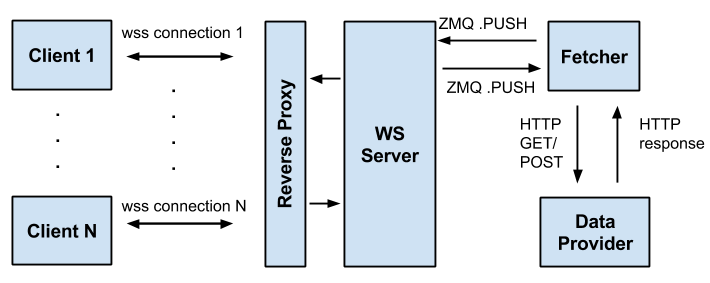
\includegraphics[width=0.8\textwidth]{images/websocketMessagingSystem}
	\caption{Structure of the WebSocket messaging system}
	\label{fig:webSocketMessagingSystem}
\end{figure}

\subsection{Clients}

A client opens up a connection with the WebSocket server and makes a request for specific keys. In the case of a chat application these keys would most likely be conversation identifiers that are kept in a persistent storage on the backend side. Different clients request different keys based on the conversations they are a part of and thus subscribed to. In the case of the WebSocket messaging system the client is simply a viewer for data generated by the data provider. The system is designed to support multiple concurrent connections between clients and the WebSocket server.

\subsection{Reverse Proxy}

The reverse proxy is used as a tunnel between the clients to the WebSocket server and provides an encrypted connection with Transport Layer Security. The load balancing capabilities of Nginx also make it possible to scale individual parts of the system which makes it possible to scale the system horizontally when bottlenecks have been identified later on in the development process. The Nginx configuration files for unencrypted and encrypted WebSocket traffic can be found in Appendix~\ref{chapter:appendix-reverseProxy}.


\subsection{WebSocket Server}

The WebSocket server listens on a specific port and establishes a WebSocket connection upon request. Further connection management is dependent on the WebSocket implementation used by the server. The Node.js WebSocket implementation used in the system is called ws\footnote{\url{https://github.com/websockets/ws}} and adds no extra functionality to the WebSocket API and protocol specifications. The aim of the project is to stay up to date with RFC 6455 while providing a simple and fast implementation of WebSocket.
\\ \\
After a WebSocket connection had been established the server is responsible for returning data associated with the key requested by a client. Either the server has the data in memory or it must request it from the fetcher using a push socket over a TCP connection using the ZeroMQ library. The communication with the fetcher goes through a ZeroMQ client which is needed in able to use the binary protocol of the library. The code for the WebSocket server can be found in Appendix~\ref{chapter:appendix-webSocketServer}.

\subsection{Fetcher}

The fetcher maintains a queue of requests made by the WebSocket server and manages a cluster of worker processes that handle HTTP requests that are mode to the data provider for requested data. This technique makes it possible to have separate processes share the same server port and take an advantage of the available cores on the host machine. A master process listens on a port, accepts new connections and distributes them to available worker processes using a round-robin scheduling algorithm \cite{nodeCluster}. The worker processes are spawned such that they can communicate with the master process via IPC and are capable of passing server handles back and forth. The master process is then responsible for managing the worker process to avoid overloading and load-balances requests from the WebSocket server to different workers processes.
\\ \\
The clustering approach allows the WebSocket messaging system to improve throughput and resource utilization when managing production workload by taking advantage of multi-core processors despite the single threaded nature of Node.js. Another advantage of this approach compared to communication patterns like polling and long-polling is that the fetcher and the data provider can be places geographically close to each other, like in the same data center, which can reduced latency. The code for the fetcher can be found in Appendix~\ref{chapter:appendix-fetcher}.
\\
\begin{figure}[h!]
	\centering
	\label{fig:webSocketMessagingSystem}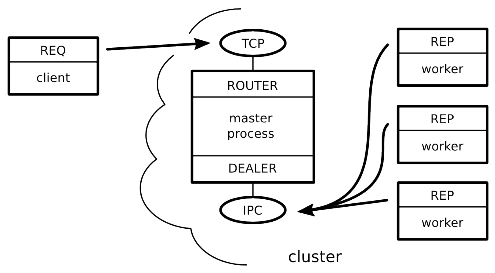
\includegraphics[width=0.7\textwidth]{images/poolOfWorkers}
	\caption{A Node.js cluster that routes requests to a pool of workers \cite{judd2008node}}
\end{figure}

\subsection{Data Provider}

The data provider serves JSON or random text and binary data over a HTTP-based API. In this implementation the data provider does not provide any meaningful data but has the purpose of simulating the data source that the WebSocket messaging system is intended to eventually use. The code for the data provider can be found in Appendix~\ref{chapter:appendix-dataprovider}.

\section{Benchmarking}

The purpose of the benchmarking tests was to figure out how many concurrent clients the messaging system could handle without dropping connections. The results can be used as a basis for capacity planning of a WebSocket-based infrastructure or used to analyse the WebSocket messaging system for further development.
\\ \\
The load test was implemented in the manner that a new client connects to the WebSocket server every two seconds and afterwards requests a 130 KB JSON file every second. The benchmarking was done for two different instance types, one with 4GB RAM  and 2 CPUs and another one with 8GB RAM and 4 CPUs. Both instances had SSD drives and were located in a data center in Frankfurt with the clients that made request being located in Iceland. Version 0.10.38 of Node.js (the minor version provided in repositories of most common Linux distributions) was used to run all the components of the system that were deployed on a Ubuntu 14.04.2 LTS OS with a 3.13.0-52 Linux kernel. The Nodetime\footnote{\url{https://nodetime.com/}} application monitoring and analytics service was for performance measurement and the \texttt{iptraf} Unix tool was used to measure network traffic.
\\ \\
The metrics of the benchmarking test were: Available memory, CPU time, V8 heap used and full garbage collections while the WebSocket messaging system was able to cope with increasing number of concurrent client connections. The duration of the tests was around ten minutes in both cases and the results can be seen in following figures. The code for the load test can be found in Appendix~\ref{chapter:appendix-loadtest}.
\\
\begin{figure}[h!]
	\centering
	\subfigure[4GB RAM / 2 CPUs]{\label{fig:freeMemory-2cpus}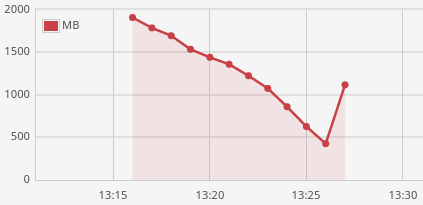
\includegraphics[width=0.49\textwidth]{images/freeMemory-2cpus}} \hfill
	\subfigure[8GB RAM / 4 CPUs]{\label{fig:freeMemory-4cpus}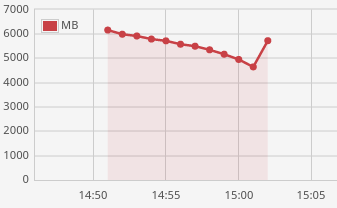
\includegraphics[width=0.49\textwidth]{images/freeMemory-4cpus}}
	\caption{Free memory (MB)}
	\label{fig:freeMemory}
\end{figure}

\noindent
Figures~\ref{fig:freeMemory-2cpus} and~\ref{fig:cpuTime-4cpus} clearly show how the memory of the instances decreases as more clients connect to the WebSocket server until the server crashes and the instances regain some of their memory. The smaller instance managed 304 concurrent connections and the larger one managed 333 ones before starting to drop client connections. Neither instance used any of its swap space so lack of physical memory was not the reason behind the connection saturation. This in an indicator that a horizontal scaling strategy might be more suitable for the messaging system than a vertical one.
\\
\begin{figure}[h!]
	\centering
	\subfigure[4GB RAM / 2 CPUs]{\label{fig:cpuTime-2cpus}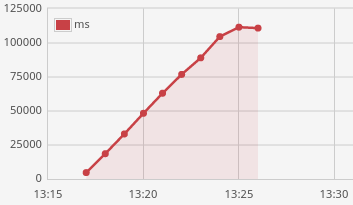
\includegraphics[width=0.49\textwidth]{images/cpuTime-2cpus}} \hfill
	\subfigure[8GB RAM / 4 CPUs]{\label{fig:cpuTime-4cpus}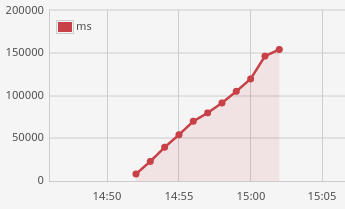
\includegraphics[width=0.49\textwidth]{images/cpuTime-4cpus}}
	\caption{CPU time  (ms)}
\end{figure}

\noindent
As can be expected the time used for processing instructions by the CPUs increase incrementally with the number of concurrent connection as shown in figures~\ref{fig:cpuTime-2cpus} and~\ref{fig:cpuTime-4cpus}. Further analysis would be required to determine exactly how the CPU time is shared between different programs on the instances. The analysis would be required to evaluate the advantage of the clustering implementation of the fetcher in messaging system. The true benefit of the worker pool used by the fetcher seems to be more related to the possibility to have concurrent network calls rather than parallel processing threads based on the figures shown before.
\\
\begin{figure}[h!]
	\centering
	\subfigure[4GB RAM / 2 CPUs]{\label{fig:v8heapUsed-2cpus}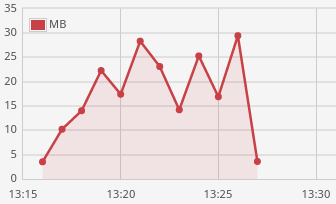
\includegraphics[width=0.49\textwidth]{images/v8heapUsed-2cpus}} \hfill
	\subfigure[8GB RAM / 4 CPUs]{\label{fig:v8heapUsed-4cpus}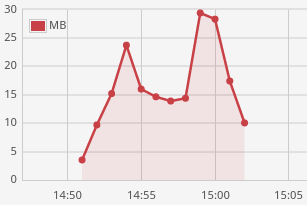
\includegraphics[width=0.49\textwidth]{images/v8heapUsed-4cpus}}
	\caption{V8 heap used (MB)}
\end{figure}

\noindent
Figures~\ref{fig:v8heapUsed-2cpus} and~\ref{fig:v8heapUsed-4cpus} show memory used for heap bookkeeping by the V8 JavaScript engine. It is hard to identify any special pattern in the figures as heap management is a low level operation with numerous different spaces so further analysis would be needed to truly understand what is going on here. A possible approach for better heap management would be to use a newer version of Node.js. Version 0.10.38 (released in March 2015) which was used for the benchmarking uses a version of the V8 JavaScript engine that was released in October 2012\footnote{\url{https://code.google.com/p/v8/source/browse/trunk/ChangeLog}}. One of the main reasons behind io.js, a community driven fork of Node.js, was the slow adoption of newer versions of the V8 JavaScript engine. Future versions of Node.js should ship with a more up do date version of the V8 JavaScript engine as the two projects have been merged.
\\
\begin{figure}[h!]
	\centering
	\subfigure[4GB RAM / 2 CPUs]{\label{fig:fullGcs-2cpus}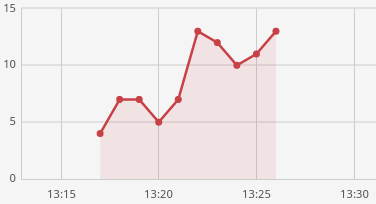
\includegraphics[width=0.49\textwidth]{images/fullGcs-2cpus}} \hfill
	\subfigure[8GB RAM / 4 CPUs]{\label{fig:fullGcs-4cpus}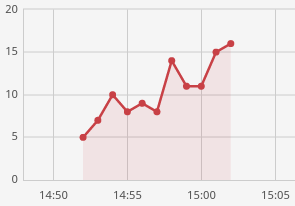
\includegraphics[width=0.49\textwidth]{images/fullGcs-4cpus}}
	\caption{Full garbage collections per minute}
\end{figure}

\noindent
As more clients connect to the WebSocket server the garbage collector kicks in more frequently which slows down overall performance because of increased memory usage. Figures~\ref{fig:fullGcs-2cpus} and~\ref{fig:fullGcs-4cpus} clearly show how the garbage collector tries to free up memory more frequently which eats up the CPU time with increasing load on the WebSocket server with more concurrent client connections. When the garbage collector is not capable of freeing up sufficient memory the clients start to lose their connections. There does not seem to be much difference in the capability of each instance with regards to successful garbage collection which is another indicator that a horizontal scaling strategy might be more suitable for the messaging system than a vertical one.
\\
\begin{table}[h!]
\centering
\begin{tabular}{lll}
\hline
	& \textbf{4GB RAM/2 CPUs}	&	\textbf{8GB RAM/4 CPUs} \\ \hline
\begin{tabular}[v]{@{}c@{}}\textbf{Maximum concurrent}\\\textbf{clients (\#)}\end{tabular} & 304	& 333 \\
\begin{tabular}[v]{@{}c@{}}\textbf{Average outgoing}\\\textbf{rate (MB/sec)}\end{tabular} & 46,34	& 47,17 \\
\hline                         
\end{tabular}
\caption{Number of concurrent client connections and the rate of data transfer}
\label{table:connectionsDatarate}
\end{table}

\noindent
The maximum number of concurrent connections and average outgoing data rate during the load test is another indicator that the computational capabilities of the instances has a small effect on the overall performance of the WebSocket messaging system. The number of concurrent clients seems to be determined by the performance of the V8 JavaScript engine as seen before. The outgoing data rate can possibly be increased by configuring the network for increased bandwidth but that largely depends on how the system is deployed. If a public cloud service is being used it can introduce an operation challenge as the control over the underlying infrastructure is often handled by the cloud infrastructure operator. Therefore it is important to choose an infrastructure for deployment that enables enough control so that it can be tuned specially for this use case. The other option would be to adjust the WebSocket messaging system to the underlying infrastructure. In either case it is important to have a good understanding of how both the system and the environment where it is deployed. The best way to achieve that understanding is to monitor the system when it has been put into production use and make required configurations as they become evident.

\section{Possible Improvements and Further Work}

The WebSocket messaging system that was presented in this chapter was intended as a prototype that could be used as the starting point for further development. One discovery of benchmarking test of the system is that there seams to be an upper limit on how many concurrent connection the WebSocket server can handle. That limitation could be bypassed with a load-balancing strategy which would be necessary if the system was to be deployed for production use. The Nginx reverse proxy server that is already a part of the system could be extended to manage load among multiple WebSocket servers whose number could be increased or decreased on demand. This implementation should be achievable with minimum adjustment to other parts of the system like depicted in figure~\ref{fig:websocketMessagingSystemLoadBalancer}. Load-balancing tests to certify the scalability of Nginx have shown that the project lives up to its high promises on high concurrency by managing up to 50,000 concurrent WebSocket connections \cite{nginxWebsocket}.
\\
\begin{figure}[h!]
	\centering
	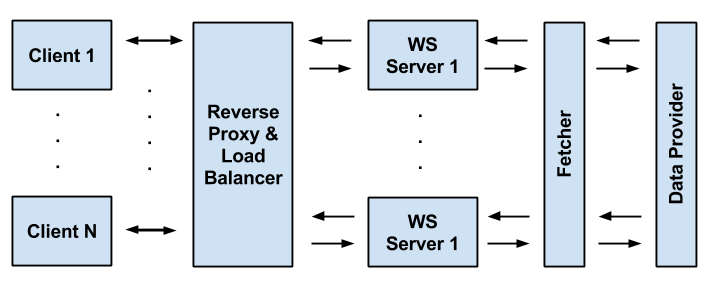
\includegraphics[width=0.8\textwidth]{images/websocketMessagingSystemLoadBalancer}
	\caption{The WebSocket messaging system with a load balancer}
	\label{fig:websocketMessagingSystemLoadBalancer}
\end{figure}

\noindent
Another possible improvement for the system would be to implement a publish-subscribe communication pattern between the WebSocet server and the data provider. This would make the fetcher redundant and could possibly increase the responsiveness of the system. The main disadvantage of this approach is that it would require modifications to the backend service which would lead to tighter coupling of the system which is in contrast with the microservices ideology. Figure~\ref{fig:websocketMessagingSystemServerPush} shows a possible structure of this of system implementation.
\\
\begin{figure}[h!]
	\centering
	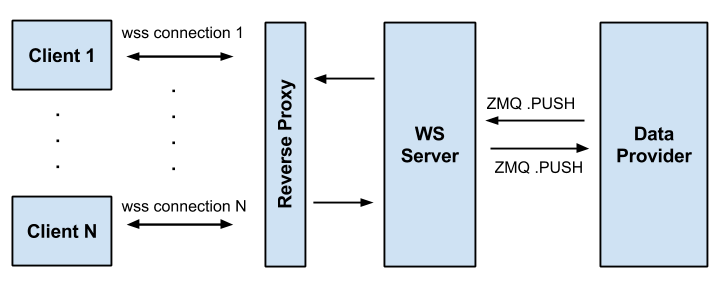
\includegraphics[width=0.8\textwidth]{images/websocketMessagingSystemServerPush}
	\caption{The WebSocket messaging system using server push}
	\label{fig:websocketMessagingSystemServerPush}
\end{figure}

\noindent
The only way to truly understand how such a system behaves is to deploy it in a production environment and monitor it thoroughly. When a piece of software, like the WebSocket messaging system, is exposed to actual usage unknown issues can be identified more rapidly and dealt with accordingly.

